% Author: Matt Toman

\chapter{History of Retinal Imaging}

\label{history_retinal_imaging}
\lhead{\emph{History of Retinal Imaging}}


\section{History and Development of Retinal Imaging Techniques}

Direct examination of the retina is prevented by the optical properties of the
eye that enable image capture and formation.  That is to say, when trying to
form a retinal image from outside via an inverse imaging transform, depiction
of the retina is actually prevented by the nature of the original transform which
results in a focused image on its surface.

If light is shone into the eye at a certain angle, a blurred reflection of the
retina can make the pupil appear to be red in colour.  This is known as
the red reflex, and has been understood for hundreds of years.  Obtaining
a focused retinal image is much more difficult, however, and requires
specialist techniques. The first successful attempt to acquire a retinal
image was performed by Jean Mery, a French physician, in 1704.
\cite{valsalva1704aure}  Mery  showed that if a live cat is submerged in
water, the vessels of its retina can be seen from the outside.
\cite{collegeoptometrists}

Czech scientist Jan Purkinje observed the fundus of a dog and later a
human eye with the use of his myopic spectacles.  Acting as a concave
mirror, they reflected light into the eye from a candle situated behind the
subject.  He also provided sketches of his own retinal vasculature, shown
in \fref{fig:retinal_drawings}. His research resulted in the realisation of the
first principles of the opthalmoscope in 1823.  This was later reinvented
by Charles Babbage in1845. \cite{flick1947centenary,keeler1997150}
Babbage was also responsible for the original concept of a programmable
computer, solidifying the link between retinal imaging and computing at an
early stage.\cite{halacy1970charles}

\begin{figure}[htbp]
\centering
  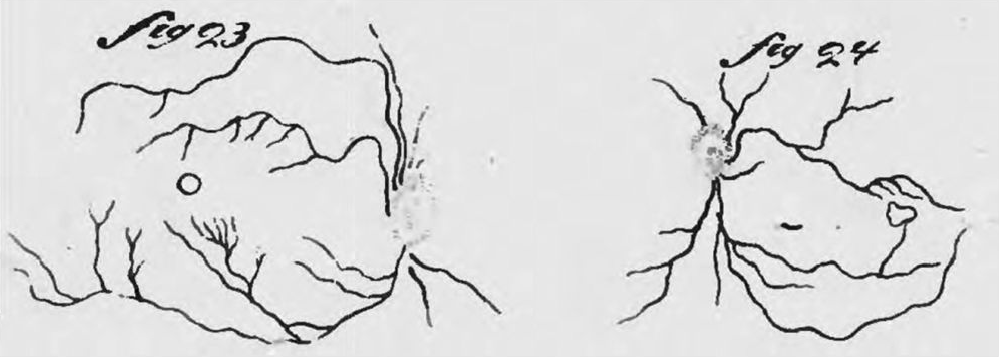
\includegraphics{figures/retinal_vasc_drawings}
\caption{Early drawings of retinal vasculature, published by Purkinje in 1823.\cite{purkinjeje}}
\label{fig:retinal_drawings}
\end{figure}

The opthalmoscope was reinvented again by von Helmholtz in 1851.  As with many other important inventions, it was not based on any radical new concepts, but was a combination of several known principles.  The fundamentals of opthalmoscopy are simple.  If the subject's eye is emmetropic, or sharp and well defined, light rays which emanate from a given point on the fundus will emerge as parallel beams.  When this beam enters the pupil of an emmetropic observer the individual rays are focused on to the observer's retina, as shown in \fref{fig:direct_opthal}.  The result is the formation of the image of the patient's retina on the observer's retina.  This is known as direct opthalmoscopy.

\begin{figure}[htbp]
\centering
  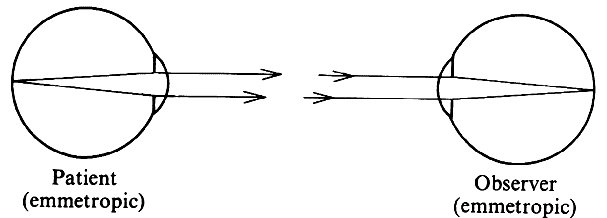
\includegraphics{figures/direct_opthalmoscopy}
\caption{Imaging in direct ophthalmoscopy. Provided the subject and the observer are both emmetropic, rays emanating from a point in the subject's fundus will emerge as a parallel beam, focused on the observer's retina.\cite{colenbrander2013principles}}
\label{fig:direct_opthal}
\end{figure}

There is a significant problem with direct ophthalmoscopy, however.  The patient's fundus has to be well illuminated for there to be sufficient light to visualise it.  Due to the optics of the eye, incident light can only reach the part of the fundus where the image of the light source falls.  Therefore the fundus can only be seen where the observed and illuminated areas overlap.  In the emmetropic eye this requires the light source and the observer's pupil to be optically aligned.

Fortunately there are several methods in which the illuminating and observing beams can be optically aligned, as shown in \fref{fig:illum_methods}.  The problem was solved by von Helmholtz with the use of a semi-reflecting mirror, made from thin pieces of glass in a parallel arrangement (A). Epkens and Ruete used a perforated concave mirror (B), which places illuminating light rays around the observation beam.  Modern-day hand held instruments now use a small mirror or a prism, which utilises the bottom half of the subject's pupil for illumination and the top half for observation (C).

\begin{figure}[htbp]
\centering
  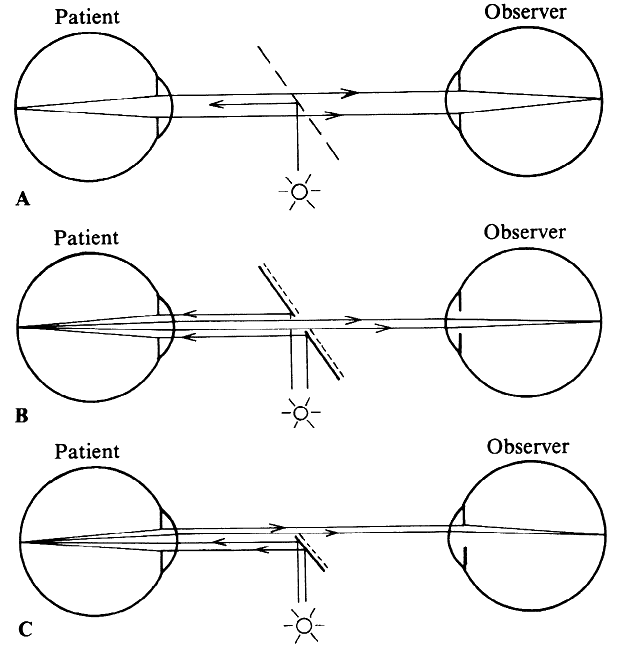
\includegraphics{figures/illumination_methods}
\caption{Illumination methods in direct opthalmoscopy. A: Semireflecting mirror (Helmholtz). B: Perforated mirror (Epkens \& Ruete). C: Prism (modern).\cite{colenbrander2013principles}}
\label{fig:illum_methods}
\end{figure}

Even with good levels of illumination, direct ophthalmoscopy suffers from a limited field of view, as shown in \fref{fig:limited_direct}.  Of the four pencils of light that emanate from the subject’s eye, points 1 and 4 cannot be seen because their directions diverge beyond the observer’s pupil.  

\begin{figure}[htbp]
\centering
  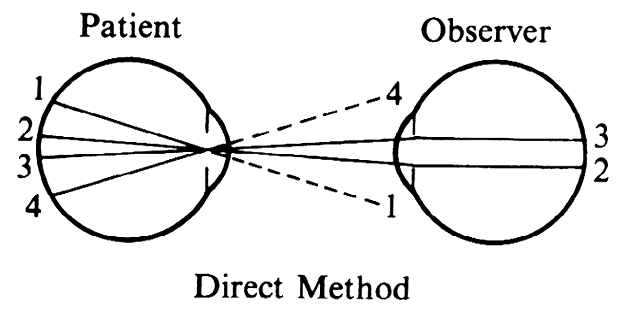
\includegraphics{figures/indirect_opthal}
\caption{The direct method suffers from a limited field of view. Pencils of light 1 and 4 do not reach the observer’s pupil.}
\label{fig:limited_direct}
\end{figure}


In order to bring these pencils of light to the observer’s pupil their direction must be altered.  This is achieved by placing a large lens between the subject’s eye and the observer’s eye, also known as indirect ophthalmoscopy.  This method, shown in \fref{fig:indirect_main}, was first introduced in 1852 by Theodore Reute.\cite{reutecgt}  There are some important implications of using an intermediate lens, making indirect ophthalmoscopy more complicated than the direct method.  The primary implication is demonstrated in the diagram, namely that the orientation of the image of the observer’s retina is inverted, a facet that can cause confusion with localisation.  

\begin{figure}[htbp]
\centering
  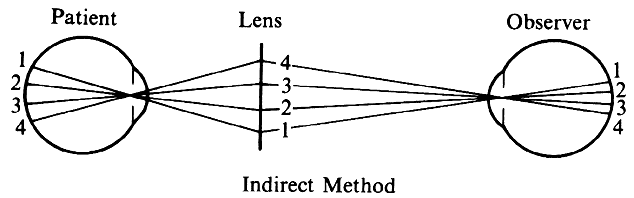
\includegraphics{figures/indirect_opthal2}
\caption{The indirect method offers an extended field of view.  Peripheral light is redirected by the lens towards the observer.}
\label{fig:indirect_main}
\end{figure}

The inspection and evaluation of the retina quickly became a routine exercise for ophthalmologists.  The first known image of the human retina, shown below in \fref{fig:human_retina} was published by the Dutch ophthalmologist van Trigt in 1853.

\begin{figure}[htbp]
\centering
  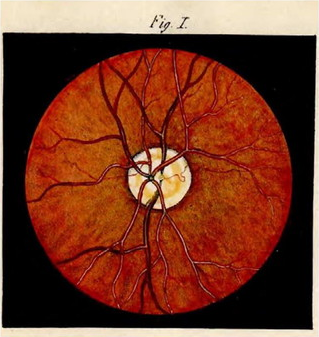
\includegraphics{figures/first_human_retina}
\caption{First known image of the human retina, drawn by Van Trigt in 1853.\cite{van1853dissertatio}}
\label{fig:human_retina}
\end{figure}

Due to the high prevalence of infectious diseases at the time, and because the ophthalmoscope necessitated the physician to be in close contact with the face of the patient, it became popular to image the eye photographically.  The first clear photographic images of the retina were obtained by German ophthalmologist Gerloff in 1891.\cite{gerloffphoto}  In 1910, a Swede named Gullstrand developed the fundus camera.  He went on to receive the Nobel prize for his invention, and the concept is still utlised to image the retina in the present day.\cite{gullstrandcamera}   has remained the primary method of retinal imaging because of how cost effective and safe it is to use.

The next crucial development was the invention of fluorescein angiographic imaging, which was first used successfully in 1961.  A fluorescent dye is injected into the bloodstream and binds to the patient's leukocytes.\cite{novotny1961method}  A fundus camera with additional narrow band filters can then be used to capture the image, an example of which is shown in \fref{fig:fluore_angio_image}.  This method has led to a better understanding of the function of retinal circulation.  However, concerns over safety have resulted in this method being slowly replaced by tomographic imaging, which utilises a penetrating wave to image by sectioning, for the diagnoses and treatments of eye diseases such as macular edema and macular degeneration.

\begin{figure}[htbp]
\centering
  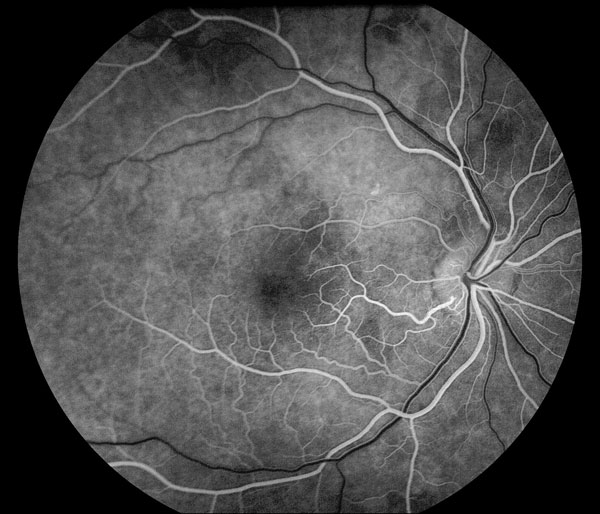
\includegraphics{figures/fluore_angio}
\caption{Normal Fluorescein Angiogram. Arterial phase illustrating sodium fluorescein dye in the retinal arteries before filling the retinal veins.\cite{medicine_uiowa}}
\label{fig:fluore_angio_image}
\end{figure}

Tomographic imaging of the retina has become common practice following the development of femtosecond lasers, super-luminescent diodes, and, most significantly, the application of optical coherence tomography (OCT) to retinal imaging.\cite{huang1991optical} This technique uses light to capture 3D images from within optical scattering media at micrometer-resolution, allowing for true 3D optical sectioning of the retina.\cite{van2007recent}

As the prevalence of diseases such as diabetes increased, along with the medical demands of an aging population, there became a clear need for more efficient image analysis techniques to facilitate screening programmes.

Retinal image analysis methods were first examined by Matsui et al in 1973. Their approach was grounded in mathematical morphology, utilising digitized slides of fluorescein angiograms of the retina, with a primary focus on vessel segmentation.\cite{matsui1973study}

Many attempts to segment other anatomical structures in the eye were made in the subsequent years, all based on the use of digitized slides. Badouin et al were the first to provide a method to detect and segment abnormal ocular structures, when in 1984 they described an image analysis method for the detection of microaneurysms, which is a characteristic symptom of diabetic retinopathy.\cite{baudoin1983automatic} Their approach also utilised digitized angiographic images.  Microaneurysms were detected via the use of a "top-hat" transform, a step-type variant of a digital image filter.\cite{sonka1998image}  

The field of retinal image analysis changed drastically in the 1990s with the development of digital retinal imaging and filter-based image analysis techniques. These advances in digital-based technology also resulted in rapidly increasing numbers of publications.



\section{Practical Difficulties in Retinal Imaging}
[ ]


Imaging the retina presents a series of unique technical problems compared
with more commonplace photography. The primary difficulties are the turbidity
of the ocular tissue (such as cataracts in the lens), the constrained aperture
size and diffraction limit as a result of the relatively small pupillary opening, the inability of
illumination and imaging light to intersect and the fundamental challenge of
representing a curved 3-D structure as a 2-D image.

A serious limitation of fundus photography is that it only obtains a 2D representation of 3D retinal tissues, projected onto the imaging plane. Attempts to deal with this resulted in the invention of new devices and techniques. Stereo fundus photography, was first described in 1964 by Allen.\cite{allen1964ocular} This new approach relied on multi-angle retinal images combined by the human observer to derive a 3D shape. Confocal scanning laser ophthalmoscopy was later developed. This innovation utilised a confocal aperture to obtain multiple images of the retina at different depths, yielding an estimate of its 3D shape. These are discussed in more detail in the following section.\cite{webb1987confocal}
The inaccuracies and shortcomings in 3-D retinal imaging
led to the development of independent tomographic scanning devices such as the OCT.

Cataracts are a symptom of age related eye changes,where 
the lens becomes opaque and thus reduces the visual field of the patient,
shown in \fref{fig:cat}. If the cataract is located over the pupil then this
biological phenomena can altogether prevent the capturing of a retinal image,
akin to covering the object of a photograph with a veil, hence blocking the
illuminating light from penetrating the outer surface of the eye and onto the
retina. This is a problem for most retinal imaging devices 
and is solved by the removal of the cataracts via surgical procedure. 

\begin{figure}[htbp]
\centering
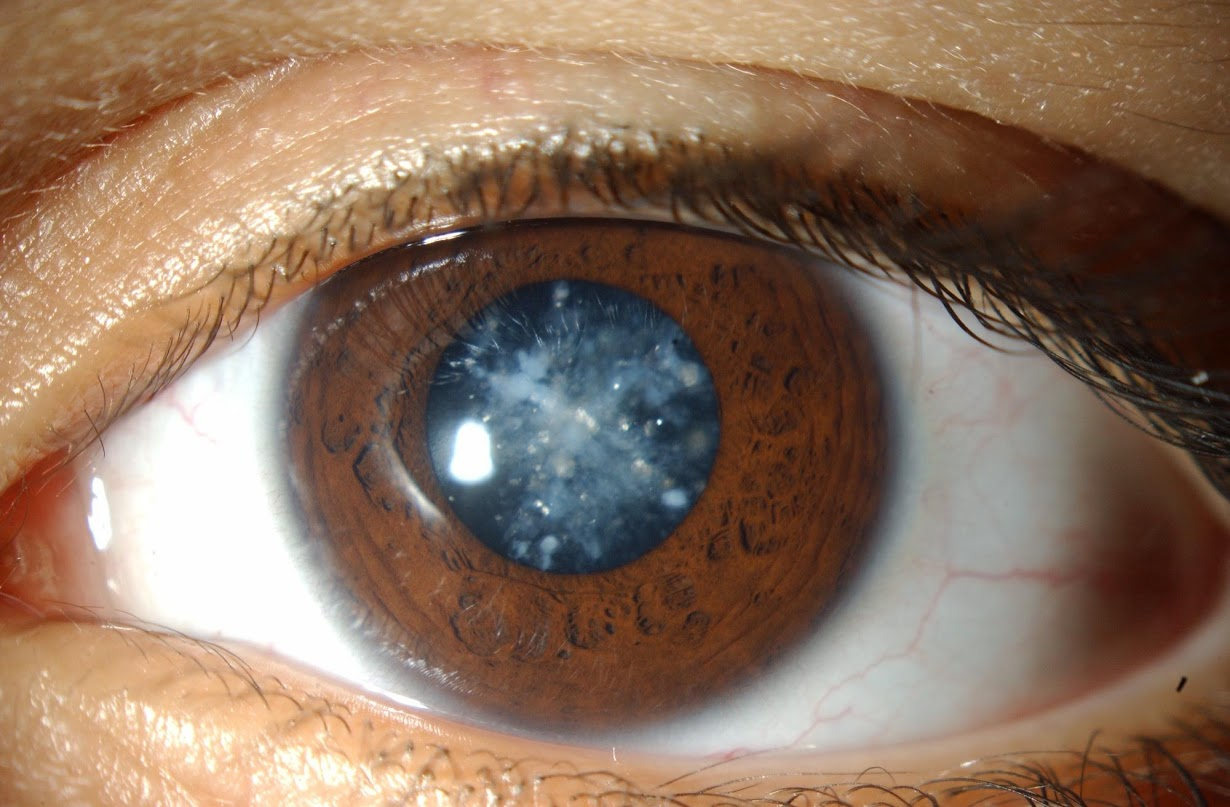
\includegraphics{figures/cataract}
\caption{Image showing the clouding of the lens as a result of a cataract}
\label{fig:cat}
   \end{figure}

Aperture size is the physical limitation of the optical system that
constrains the amount of light available for capture through a lens,
where available light is proportional to aperture area, which is in
turn related to the optical system is shown in \eref{eq:optical_system}

\begin{equation}
A = \pi({\frac{f}{2N}})^2
\label{eq:optical_system}
\end{equation}

where A is the area of the aperture, N is the f-number (ratio of lens'
focal length to diameter of entrance pupil) and f is the focal length
of the lens. This relationship is applicable to the case of the fundus
camera, where expanding the pupillary opening reduces this constraint.
To maximise the pupillary opening the patient is photographed in a dark
room where pupil diameter can be between 3-8mm, dependent on age. If this
effect is insufficient then an increased pupil diameter is chemically
induced through the use of mydriatic eye drops, which relax the constrictive
nerves, shown in \fref{fig:myd}.

\begin{figure}[htbp]
\centering
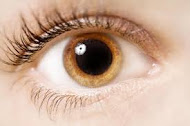
\includegraphics{figures/mydriasis}
\caption{Image showing the effect of mydriatic medicine on the pupillary opening}
\label{fig:myd}
   \end{figure}

The diffraction limit of vision, as was shown in the previous section, 
acts as a fundamental limit to the achievable resolution of vision. This is also
applicable to retinal imaging as the optical system is simply reversed, with 
the pupil again acting as a diffraction grating. To reduce this effect imaging
devices are placed as close as possible to the eye, with most standard 
instruments capable of an optical resolution of around 20 microns.

As the pupil is the only opening through which the retina can be
observed, light is required to enter and leave through the same
optical path, consequently care has to be taken to avoid ray overlap
otherwise the image will have reduced or zero contrast. Gullstrand
first introduced this idea in 1910, where he stated that to avoid
scattering between the two beams they must be entirely unconnected
across the optical path. He further specified that bright corneal
reflections are the result of scattering on the corneal plane,
whereas scattering from lens surfaces and opacities occur as the
light rays penetrate the lens. This challenge is overcome in
imaging devices and will be discussed in greater detail in the
following section.

